% --------------------------------------------------------------
%                           Set Up
% --------------------------------------------------------------
 
\documentclass[12pt]{article}
 
\usepackage[margin=1in]{geometry} 
\usepackage{amsmath,amsthm,amssymb}
\usepackage{listings}
\usepackage{xcolor}
\usepackage{graphicx}
\usepackage{subcaption}
\usepackage{listings}
\usepackage{xcolor}
 
\definecolor{codegreen}{rgb}{0,0.6,0}
\definecolor{codegray}{rgb}{0.5,0.5,0.5}
\definecolor{codepurple}{rgb}{0.58,0,0.82}
\definecolor{backcolour}{rgb}{0.95,0.95,0.92}
 
\lstdefinestyle{mystyle}{
    backgroundcolor=\color{backcolour},   
    commentstyle=\color{codegreen},
    keywordstyle=\color{magenta},
    numberstyle=\tiny\color{codegray},
    stringstyle=\color{codepurple},
    basicstyle=\ttfamily\footnotesize,
    breakatwhitespace=false,         
    breaklines=true,                 
    captionpos=b,                    
    keepspaces=true,                 
    numbers=left,                    
    numbersep=5pt,                  
    showspaces=false,                
    showstringspaces=false,
    showtabs=false,                  
    tabsize=2
}
 
\lstset{style=mystyle}
 
\definecolor{codegreen}{rgb}{0,0.6,0}
\definecolor{codegray}{rgb}{0.5,0.5,0.5}
\definecolor{codepurple}{rgb}{0.58,0,0.82}
\definecolor{backcolour}{rgb}{0.95,0.95,0.92}
\definecolor{deepblue}{rgb}{0,0,0.5}
\definecolor{deepred}{rgb}{0.6,0,0}
\definecolor{deepgreen}{rgb}{0,0.5,0}
 
\lstdefinestyle{mystyle}{
    backgroundcolor=\color{backcolour},   
    commentstyle=\color{codegreen},
    keywordstyle=\color{deepred},
    numberstyle=\tiny\color{codegray},
    stringstyle=\color{deepblue},
    basicstyle=\ttfamily\footnotesize,
    breakatwhitespace=false,         
    breaklines=true,                 
    captionpos=b,                    
    keepspaces=true,                 
    numbers=left,                    
    numbersep=5pt,                  
    showspaces=false,                
    showstringspaces=false,
    showtabs=false,                  
    tabsize=2
}
 
\lstset{style=mystyle}
 
\newcommand{\N}{\mathbb{N}}
\newcommand{\Z}{\mathbb{Z}}
 
\newenvironment{theorem}[2][Theorem]{\begin{trivlist}
\item[\hskip \labelsep {\bfseries #1}\hskip \labelsep {\bfseries #2.}]}{\end{trivlist}}
\newenvironment{lemma}[2][Lemma]{\begin{trivlist}
\item[\hskip \labelsep {\bfseries #1}\hskip \labelsep {\bfseries #2.}]}{\end{trivlist}}
\newenvironment{exercise}[2][Exercise]{\begin{trivlist}
\item[\hskip \labelsep {\bfseries #1}\hskip \labelsep {\bfseries #2.}]}{\end{trivlist}}
\newenvironment{problem}[2][Problem]{\begin{trivlist}
\item[\hskip \labelsep {\bfseries #1}\hskip \labelsep {\bfseries #2.}]}{\end{trivlist}}
\newenvironment{question}[2][Question]{\begin{trivlist}
\item[\hskip \labelsep {\bfseries #1}\hskip \labelsep {\bfseries #2.}]}{\end{trivlist}}
\newenvironment{corollary}[2][Corollary]{\begin{trivlist}
\item[\hskip \labelsep {\bfseries #1}\hskip \labelsep {\bfseries #2.}]}{\end{trivlist}}

\newenvironment{solution}{\begin{proof}[Solution]}{\end{proof}}

\setlength\parindent{0pt}
 
\begin{document}
 
% -------------------------------------------------------------- 
%                         Start here
% --------------------------------------------------------------
 
\title{Homework 2}
\author{Timothy Holmes\\ %replace with your name
PHY 475 Introduction to Cosmology}

\maketitle

\section*{Problem 4.4}

The critical mass density of the universe is found using the equation

$$
\rho_{c} = \frac{3H^{2}}{8\pi G} = \frac{\epsilon_{c,0}}{c^2} = (8.7 \pm 0.5)*10^{-27} kg*m^{-3}.
$$

The number density, mass, and critical mass show that $\rho_{c,0} = n*m$. Therefore, the number density of baseballs can be found using

$$
n = \frac{(8.7 \pm 0.5)*10^{-27} kg*m^{-3}}{0.145 kg} = 6*10^{-26}m^{-3}
$$

The equation for line of site was defined in chapter two by the Author. The equation for this is 

$$
\lambda = \frac{1}{n\pi r^2} = \frac{1}{\pi * (0.0369 m)^{2}} = 3.89*10^{27}m
$$

\section*{Problem 4.5}

The equation equation of state is given as $P = w\epsilon$. Where the total energy density can be expressed as $\epsilon = n E_{p}$. Therefore, the equation of state can be expressed as

$$
w = \frac{P}{nE_{p}}.
$$

The fluid equation is given as $\dot{\epsilon} + 3(\dot{a}/a(\epsilon + P) = 0$. Since $\epsilon$ has been solved for, the fluid equation can now be expressed as 

$$
P = -nE_{p} - \frac{a}{3\dot{a}}\Big(\frac{d}{dt}(nE_{p})\Big)
$$

which can be wrote as

$$
P = -nE_{p} - \frac{a}{3}\Big(\frac{dn}{da}E_{p} + n\frac{dE_{p}}{da}\Big)
$$

Furthermore,

$$
P = -nE_{p} - \frac{a}{3}\Big(-\frac{3n_{0}E_{p}}{a^{4}} + \frac{n}{2}(m^{2}c^{4} + p^{2}c^{2})^{1/2}\Big(\frac{2p^{2}c^{2}}{a^{2}}\Big)\Big)
$$

which deduces down to 

$$
P = \frac{np^{2}c^{2}}{E_{p}3}.
$$

Above we had that $w = P/nE_{p}$ and $P = np^{2}c^{2}/E_{p}3$, therefore,

$$
w = \frac{p^{2}c^{2}}{3E^{2}_{p}}.
$$

Let us now consider the scenario when $a \rightarrow 0$ and $p \rightarrow \infty$.
Expanding what was found for $w$, 

$$
w = \frac{c^{2}}{3(c^{2} + m^{2}c^{4}/p^{2})}.
$$

If $p \rightarrow \infty$ then the $m^{2}c^{4}/p^{2}$ will got to zero. This reduces to 

$$
w = \frac{c^{2}}{3c^{2}}.
$$

The $c^{2}$ terms will cancel out leaving $w = 1/3$, our desired answer. Now, the scenario when $a \rightarrow \infty$ and $p \rightarrow 0$. Similar to the scenario above we have the equation for $w$ as

$$
w = \frac{c^{2}p^{2}}{3p^{2}(c^{2} + m^{2}c^{4}/p^{2})}.
$$

If $0$ is entered in for $p$ the equation becomes

$$
w = \frac{c^{2}*0}{3*0(c^{2} + m^{2}c^{4}/p^{2})} = 0.
$$

\section*{Problem 5.1}

The redshift z for a spatially flat, single-component universe is written in the following relation as 

$$
1 + z = \frac{a(t_{0})}{a(t_{e})} = \Big(\frac{t_{0}}{t_{e}}\Big)^{2/(3+3w)}.
$$

It is evident that $t_{0}$ time observed and $t_{e}$ time emitted are both times. Thus, any derivative taken with time will affect $t_{e}$ and $t_{0}$. What this really tells us is that we see some change in time at $t_{e}$ and in some other time $t_{0}$. Therefore, if we take the derivative of the equation defined above we have to use the quotient rule since we have $a(t_{0})/a(t_{e})$. The derivative of the redshift equation with respect to $t_{0}$ is 

$$
\frac{dz}{dt_{0}} = 
\frac{a(t_{e})
\frac{da(t_{0})}{dt_{0}} -
a(t_{0})
\frac{da(t_{e})}{dt_{0}}
}
{
a(t_{e})^{2}
}
$$

The variable $a$ can be wrote as $a = 2/3(1 + w)$. Taking the derivative with respect to time gives 

$$
\dot{a}(t) = \frac{2}{3 + 3w}\frac{a(t)}{t}.
$$

Other useful equations include $t_{0} = 2/(3 + 3w)1/H_{0}$, $dt_{0}/dt_{e} = (1 + z)$, and finally $a(t_{0})/a(t_{e}) = 1/(1 + z)$. Using these we can reduced the equation above to 

$$
\frac{dz}{dt_{0}} = H_{0}\Big(1 - (1+z)^{3+3w/2}\frac{1}{1+z}\Big)(1+z)
$$

and in its final form

$$
H_{0}(1+z) - H_{0}(1+z)^{3+3w/2}.
$$

In the exponent we have the equation 

$$
\frac{3 + 3w}{2} = 1 \; \; \; \; \;  w = -\frac{1}{3}.
$$

If $w < -1/3$ then $ (3 + 3w)/2$ is less than 1 and the redshift will increase with time $t_{0}$. If $w > -1/3$ then $ (3 + 3w)/2$ is greater than 1 and the redshift will decrease with time $t_{0}$. So $w < -1/3$ is needed.

\section*{Problem 5.3}

For a positively cured universe with matter in it, the Friedmann equation is given as

$$
\frac{\dot{a}^{2}}{H^{2}_{0}} = \frac{\Omega_{0}}{a} + (1 - \Omega_{0}).
$$

Ryden says that if we want to know the age of the universe we use equation 5.89 in the book given as

$$
H_{0}t = \int_{0}^{a}\frac{da}{[\Omega/a + (1 + \Omega_{0}]^{1/2}}
$$

where $a$ is the scale factor. Note that we care about the age of this universe in the present day, now. Recall that the scale factor at the present time is $a = 1$. Therefore, we get that the definite integral is 

$$
H_{0}t = \int_{0}^{1}\frac{da}{[\Omega/a + (1 + \Omega_{0}]^{1/2}}.
$$

With the use of an integral table or wolfram the solution to this integral becomes

$$
H_{0}t = \frac{1}{(1 - \Omega_{0})} - \frac{\Omega_{0} * sinh^{-1}\Big(\sqrt{\frac{1}{\Omega_{0}} - 1}\Big)}{(1 - \Omega_{0})^{3/2}}
$$ 

\begin{figure}[h!]
    \centering
    \subfloat[Figure 1]{{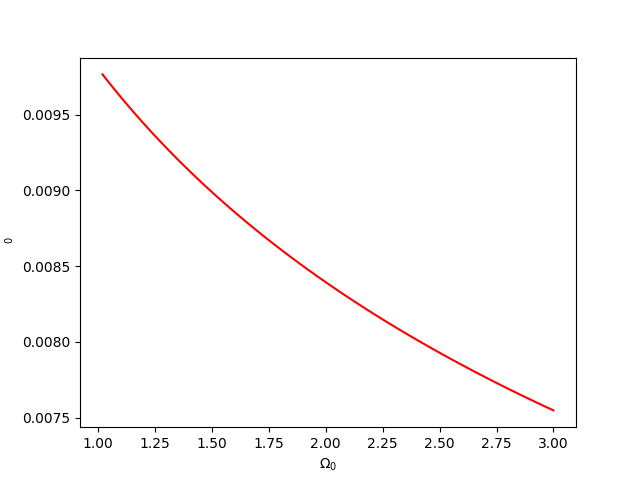
\includegraphics[width=5.7cm]{figure1.png} }}%
    \qquad
    \subfloat[Figure 2]{{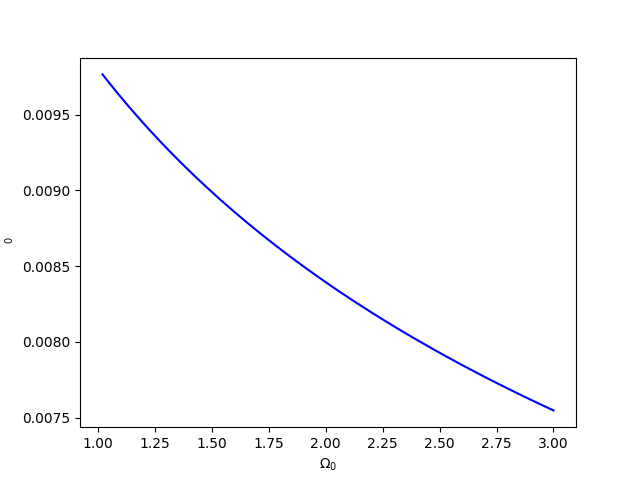
\includegraphics[width=5.7cm]{figure2.png} }}%
    \caption{Figure 1a on the left is graphed using the equation given in the book. The Figure 1b on the right is the equation solved for using the definite integral above.}%
    \label{fig:example}%
\end{figure}


Figure 1 above shows that even though the solution that was found from the definite integral above differs from the equation the book gives, the same graph is produced. The book gives the equation in the form of 

$$
H_{0}t_{0} = \frac{\Omega_{0}}{2(1 - \Omega_{0})^{3/2}}cos^{-1}\Big(\frac{2 - \Omega_{0}}{\Omega_{0}}\Big) - \frac{1}{1 - \Omega_{0}}.
$$

The differences between this equation and the equation solved for is that there is a $\sqrt{1/\Omega_{0} - 1}$. Since the $\Omega_{0}$ values used to plot are greater than 1, the values produced by this equation are both real and imaginary. If we choose to ignore the imaginary number and focus on the real numbers, this equation produces the same results as the equation gave in the book.



\section*{Problem 5}

Consider a flat universe with a single component characterized by the equation of state parameter, $w = -1$.




\subsection*{a.}

The Friedmann equation is gave in the beginning of chapter 5 with equation 5.1 as

$$
\Big(\frac{\dot{a}}{a}\Big)^{2} = \frac{8\pi G}{3c^{2}}\epsilon_{\Lambda} - \frac{kc^{2}}{R^{2}_{0}a^{2}}.
$$

For a positively curved universe $k=1$, for a negatively curved universe $k=-1$, and for a flat universe $k=0$. When $k=0$ the then $0c^{2}/R^{2}_{0}a^{2} = 0$. This reduces the Friedmann equation to 

$$
\dot{a}^{2} = \frac{8\pi G}{3c^{2}}\epsilon_{\Lambda} a^{2}.
$$

\subsection*{b.}

Taking the square of both sides and dividing $a$ to the LHS gives 

$$
H_{0} \equiv \Big(\frac{\dot{a}}{a}\Big)_{t=t_{0}} = \sqrt{\frac{8\pi G \epsilon_{\Lambda}}{3c^{2}}}.
$$

\subsection*{c.}

Since 

$$
H_{0} = \sqrt{\frac{8\pi G \epsilon_{\Lambda}}{3c^{2}}}
$$

the equation can be written as

$$
\dot{a} = H_{0}a.
$$

Integrating this equation such that 

$$
\frac{da}{dt} = H_{0}a \rightarrow \int dt = \int_{t_{0}}^{t} \frac{da}{H_{0}a}.
$$

This results in 

$$
a(t) = ln(H_{0}(t - t_{0}))
$$

and finally,

$$
a(t) = e^{H_{0}(t-t_{0})}.
$$


\section*{Appendix}

\begin{lstlisting}[language=Python, caption= Problem 5.3 plotting code]
import numpy as np
import matplotlib.pyplot as plt


omega_0 = np.linspace(1.0, 3.0, 100, dtype=complex)
H_0 = 68


# Equation found in the book
t0 = np.zeros(len(omega_0))
for i in range(0, len(omega_0)):
    t0[i] = ( ( (omega_0[i]/(2 * (omega_0[i] - 1)**(3/2))) 
        * np.arccos((2 - omega_0[i])/omega_0[i]) 
        - (1/(omega_0[i] - 1)) )/H_0 )


plt.plot(omega_0, t0, 'r')
plt.xlabel(r"$\Omega_{0}$")
plt.ylabel(r"$\t_{0}$")
plt.savefig('./figure1.png')
plt.show()


# Equation solved for by wolfram/integral table
t0 = np.ones(len(omega_0),dtype=complex)
for i in range(0, len(omega_0)):
    t0[i] = ((1/(1 - omega_0[i])) - ((omega_0[i] 
        * np.arcsinh(np.sqrt((1/omega_0[i]) 
        - 1)))/((1 - omega_0[i])**(3/2))))/H_0


plt.plot(omega_0, t0, 'b-')
plt.xlabel(r"$\Omega_{0}$")
plt.ylabel(r"$\t_{0}$")
plt.savefig('./figure2.png')
plt.show() 
\end{lstlisting}



% --------------------------------------------------------------
%                           End Document.
% --------------------------------------------------------------
 
\end{document}

